\chapter{Die Siebformel}

\begin{satz}[Siebformel / Prinzip der Inklusion/Exklusion]
    Für endliche Mengen $A_1, A_2, ... , A_n$ mit $ n \geq 2$ gilt:
    $$\left\lvert \bigcup^{n}_{i = 1} A_i \right\rvert = \sum_{l = 1}^{n}(-1)^{l+1} \sum_{1 \leq i_1 < ... < i_l \leq n} \left\lvert A_{i_1} \cap ... \cap A_{i_l}\right\rvert$$
    In Worten: Alle Schnitte von einer \textit{ungeraden} Anzahl von Ereignissen \textit{addiert} man, alle Schnitte
    von einer \textit{geraden} Anzahl von Ereignissen \textit{substrahiert} man.
\end{satz}
\bigskip

Man kann sich diese Formel oft einfacher visualisieren als beschreiben: Auf folgender Grafik
kann man sich vergewissern, dass jede der sieben Teilmengen genau einmal gezählt wird:

\begin{figure}[h]
    \centering
    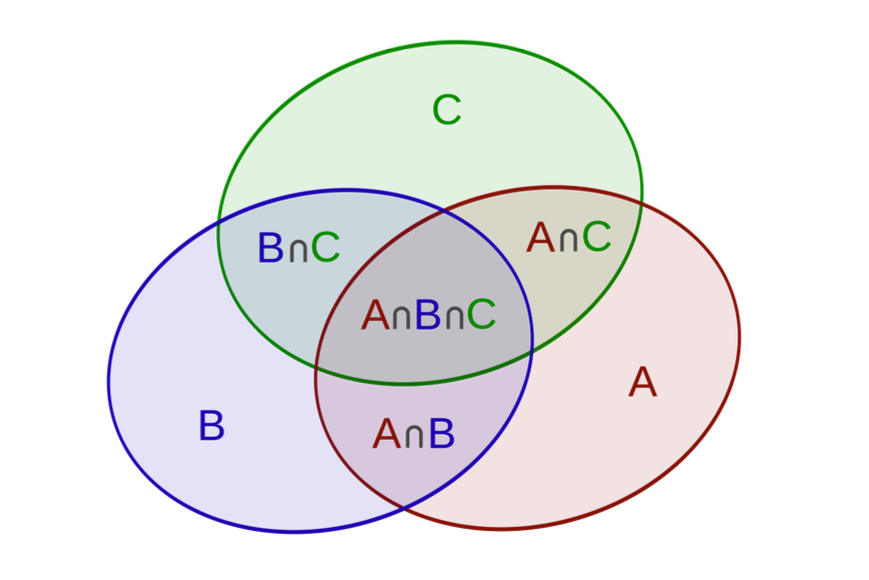
\includegraphics[width=9cm]{inclusion_exclusion.png}
    \caption{Beispiel Inklusion/Exklusion mit n = 3}
\end{figure}

$$\left\lvert \bigcup^{3}_{i = 1} A_i \right\rvert = \sum_{l = 1}^{3}\left\lvert A_l\right\rvert - \left\lvert A_1 \cap A_2 \right\rvert - \left\lvert A_2 \cap A_3 \right\rvert - \left\lvert A_1 \cap A_3 \right\rvert + \left\lvert A_1 \cap A_2 \cap A_3\right\rvert$$